\documentclass[12pt]{article}
% load packages
\usepackage{amssymb,amsmath,amsfonts,geometry,graphicx,color,setspace,natbib,hyperref}
\usepackage{kpfonts}
%\usepackage{libertine}
%\usepackage[osf,sc]{mathpazo}
%\usepackage{lipsum}
%\usepackage{newpxtext,newpxmath}
\usepackage[tableposition=top, labelfont=bf]{caption}
\usepackage{booktabs}
\usepackage[flushleft]{threeparttable}
%\usepackage{subcaption}
\usepackage{siunitx}
%\usepackage[capposition=top]{floatrow}
\usepackage[table,xcdraw]{xcolor}
\usepackage{placeins}
\usepackage{lineno}


\usepackage{natbib}
\bibliographystyle{plainnatsw}

\usepackage{tabularx} % in the preamble
\usepackage{dsfont}
\usepackage{wrapfig}
\usepackage[nameinlink,capitalise]{cleveref}
\newcommand{\crefrangeconjunction}{--}

\usepackage{caption}
\DeclareCaptionFont{xipt}{\bfseries\fontfamily{qag}\selectfont}
\usepackage[font=xipt, labelfont=bf, textfont=normalfont]{caption}

%\renewcommand{\thesubfigure}{\Alph{subfigure}}
%\captionsetup[subfigure]{font={bf,large}, labelformat=simple, skip=1pt, singlelinecheck=false}

\usepackage{siunitx}
\sisetup{
  per-mode=symbol,
  group-separator={,}
  %group-four-digits
}
\DeclareSIUnit{\ugpcm}{\micro\gram\per\cubic\meter}


\onehalfspacing
\geometry{left=1.25in,right=1.25in,top=1.0in,bottom=1.0in}
%\interfootnotelinepenalty=\@M

% sections options
\usepackage{titlesec}
\titleformat*{\section}{\fontfamily{qag}\selectfont\bfseries\LARGE}
\titleformat*{\subsection}{\fontfamily{qag}\selectfont\bfseries\large}
\titleformat*{\subsubsection}{\fontfamily{qag}\selectfont\bfseries\normalsize}
\usepackage{color, colortbl}
\definecolor{Gray}{gray}{0.9}
% color options
\definecolor{cerulean}{rgb}{0.0, 0.48, 0.65}
\definecolor{vermilion}{rgb}{0.89, 0.26, 0.2}
\hypersetup{
    colorlinks,
    linkcolor={cerulean},
    citecolor={cerulean},
    urlcolor={cerulean}
}
% fix color of brackets for citations
\bibpunct{\textcolor{cerulean}{(}}{\textcolor{cerulean}{)}}{,}{a}{}{;}

% load abstract package
\usepackage{abstract}
\renewcommand{\abstractnamefont}{\bfseries\fontfamily{qag}\selectfont}
\usepackage{epigraph}
\setlength\epigraphrule{0pt}
%\newfloatcommand{capbtabbox}{table}[][\FBwidth]

%change space in enumerates
\newenvironment{senumerate}{\enumerate\addtolength{\itemsep}{-10pt}}{\endenumerate} %espace entre les enumerate 

\usepackage{pdflscape} % landscape page
%\usepackage{changepage} % change margins for specific pages
\usepackage{sidenotes} 

\usepackage[T1]{fontenc}
\usepackage{inconsolata}

\usepackage[symbol]{footmisc}


\renewcommand{\thefootnote}{\fnsymbol{footnote}}


\makeatletter
\AtBeginDocument{
\renewcommand\NAT@open{\color{cerulean}(}}
\makeatother

%\usepackage{xurl}

\setstretch{1.5}

%----------------------------------------------------------------------

% DOCUMENT STARTS

%----------------------------------------------------------------------

\begin{document}

%----------------------------------------------------------------------

% TITLE PAGE

%----------------------------------------------------------------------

\begin{titlepage}
\vspace*{-2cm}
\begin{flushleft}
\Huge\fontfamily{qag}\selectfont\textbf{Unconfounded but Inflated Causal Estimates\footnote[2]{\textbf{Comments and suggestions are highly welcome.} We are very grateful to Hélène Ollivier and Jeffrey Shrader for their guidance on this project. Many thanks to Jesse McDevitt-Irwin, José Luis Montiel Olea, Claire Palandri, as well as Jeffrey Shrader's lab members for helpful comments and seminars participants at Columbia and Thomas Piketty's lunch seminar at PSE for their feedback.}}
\end{flushleft}
\renewcommand{\thefootnote}{\arabic{footnote}}
\begin{flushleft}
{\large
Vincent Bagilet\footnote{Columbia University, New York, USA. Email: \url{vincent.bagilet@columbia.edu}}\\[3pt] 
}
\\ [0.3cm] 
\normalsize{March 1st, 2022} \\
}

\end{flushleft}
\begin{center}
{\bfseries\LARGE  \color{cerulean}[Preliminary Work]}
\end{center}
\begin{abstract}
\noindent Convincing research designs make empirical economics credible. To avoid confounding, quasi-experimental studies focus on specific sources of variation. This often leads to a reduction in statistical power. Yet, published estimates can overestimate true effects sizes when power is low. Using fake data simulations, we first show that for all causal inference methods, there can be a trade-off between confounding and exaggerating true effect sizes due to a loss in power. We then discuss how reporting statistical power calculations could help address this issue.

\bigskip
\end{abstract}
\setcounter{page}{0}
\thispagestyle{empty}
\end{titlepage}

\renewcommand{\thefootnote}{\arabic{footnote}}

%------------------------------------------------------------------------------

% SECTION INTRODUCTION 

%------------------------------------------------------------------------------

One of the main challenges in empirical economics is to reduce confounding to identify causal effects. Identifications strategies based on Regression Discontinuity (RDD), Instrumental Variable (IV) and Difference-in-Differences (DID) can help achieve this goal. To do so, these strategies only use part of the variation in the data. They exploit the exogenous part of the variation in the treatment or decrease the sample size by only considering observations for which the as-if random assumption is credible. By reducing the variation, these methods also decrease the statistical power, that is to say the probability of rejecting the null hypothesis of no effect when it is false. This could create a tension between statistical power and reducing
confounding.



In settings with low power, statistically significant estimates will exaggerate the true effect size \citep{ioannidis_why_2008, gelman_beyond_2014}. Only estimates at least two standard errors away from zero will be statistically significant at the 5\% level. In under-powered studies, these estimates make up a selected sub-sample of all estimates, located in the tails of the distribution of all possible estimates. The average of these statistically significant estimates will differ from the true effect, located at the center of the distribution if the estimator is unbiased. When power is low, obtaining a statistically significant estimate from an unbiased estimator does not guarantee that it will be close to the true effect. 

Furthermore, a large literature has underlined the existence of a publication bias towards estimates that are statistically significant \citep[for instance]{rosenthal_file_1979, andrews_identification_2019, abadie_statistical_2020, brodeur_methods_2020}. This statistical significance filter can lead published estimates from under-powered studies to greatly exaggerate true effect sizes. \cite{gelman_beyond_2014} calls this inflation of significant estimates type M (Magnitude) error. The exaggeration of significant estimates can be computed as the expected value of statistically significant estimates over the true effect. It increases when power decreases \citep{lu_note_2019, zwet_significance_2021}.
    
This issue partly explains the current replication crisis affecting various fields such as economics, epidemiology, medicine or psychology \citep{button_power_2013, open_science_collaboration_estimating_2015, camerer_evaluating_2016, chang_is_2022}. Even in experimental economics, with a high level of control and an arguable absence of confounders, estimates published in top economic journals have failed to replicate. \cite{camerer_evaluating_2016} replicated 18 laboratory experiments and found that the effect size of original studies was on average 1.5 times larger than the replicated one. If we assume that the point estimates obtained in the replication studies represent the true effect, 44\% of the original studies would not reach the conventional 80\% power threshold. The treatment allocation in these under-powered studies may have by chance or through researchers' degrees of freedom produced estimates in the tails of the distribution, making them more likely to be published. 

Quasi-experimental studies could be more prone to this issue since statistical power is not central to the analysis in current practices. Despite usually large sample sizes, \cite{ioannidis_power_2017} concernedly finds that the median statistical power in a wide range of economic studies is no more than 18\% and that nearly 80\% of estimates may be exaggerated by a factor of two. Understanding the determinants of low power is key to avoid the inflation of published estimates. 




A large literature has underlined the existence of a publication bias towards estimates that are statistically significant \citep[for instance]{rosenthal_file_1979, andrews_identification_2019, abadie_statistical_2020, brodeur_methods_2020}. This statistical significance filter can lead published estimates from under-powered studies to greatly exaggerate true effect sizes \citep{ioannidis_why_2008, gelman_beyond_2014}. 

This can be at first sight counter-intuitive. To be statistically significant at the 5\% level, estimates must be at least two standard errors away from zero. 

In under-powered studies, these estimates make up an even more selected sub-sample of all estimates, located in the tails of the distribution of all possible estimates. The average of these statistically significant estimates will differ from the true effect, located at the center of the distribution if the estimator is unbiased. When power is low, obtaining a statistically significant estimate from an unbiased estimator does not guarantee that it will be close to the true effect. \cite{gelman_beyond_2014} calls this inflation of significant estimates type M (Magnitude) error. The exaggeration of significant estimates can be computed as the expected value of statistically significant estimates over the true effect. It increases when power decreases \citep{lu_note_2019, zwet_significance_2021}.
    
This issue partly explains the current replication crisis affecting various fields such as economics, epidemiology, medicine or psychology \citep{button_power_2013, open_science_collaboration_estimating_2015, camerer_evaluating_2016, chang_is_2022}. Even in experimental economics, with a high level of control and an arguable absence of confounders, estimates published in top economic journals have failed to replicate \cite{camerer_evaluating_2016}. Quasi-experimental studies could be more prone to this issue since statistical power is not central to the analysis in current practices. Despite large sample sizes, \cite{ioannidis_power_2017} finds that the median statistical power in a wide range of economic studies is no more than 18\% and that nearly 80\% of estimates may be exaggerated by a factor of two. Understanding the determinants of low power is key to avoid the inflation of published estimates. 

% goal of this study
In this paper, we show that design choices in quasi-experimental studies can be seen as a trade-off between avoiding confounding and overestimating true effect sizes due to a resulting loss in power. To limit the threat of confounding, causal inference methods discard variation in the treatment. It can lead to a reduction in statistical power. Due to the statistical significance filter, the resulting published estimates could be inflated and thus misleading. 

% what we actually do
In the first section of this paper, we illustrate the existence and consequences of this trade-off using fake-data simulations based on examples drawn from education, labor, environmental and political economics. We consider separately the main causal inference methods used in the economics literature: selection on observables through matching, RDD, IV and. For each identification strategy we discuss the key factors affecting the confounding / exaggeration trade-off.  When assuming that all confounders are measured, matching prunes treated units that cannot be matched to untreated ones. In RD designs, while the initial sample size may be large, we discard part of the variation by only considering observations within the bandwidth, decreasing the effective sample size. In an IV setting, we only use the treatment variation explained by the instrument. In DID event studies, the variation used to identify an effect sometimes only comes from a limited number of treated observations.

In the second section of the article, we discuss solutions to assess whether statistically significant estimates from observational studies could be inflated. We advocate reporting power calculations. They can be computed before and after the analysis is carried out. By approximating the data generating process, prospective power simulations help identify the design parameters affecting power \citep{gelman_regression_2020, black_simulated_2021}. Retrospective power calculations allow to evaluate whether a study would have enough power to confidently estimate a range of smaller but credible effect sizes \citep{gelman_beyond_2014, stommes_reliability_2021}. Our companion \href{https://vincentbagilet.github.io/causal_inflation/}{website} describes in details how such solutions can be implemented. 

% first contribution
Our paper contributes to three strands of the literature. First, the idea that causal identification estimators, while unbiased, may be imprecise is not new; this is the well-known bias/variance trade-off \citep{imbens_optimal_2012, deaton_understanding_2018, hernan_causal_2020, ravallion_should_2020}. In under-powered studies, resulting estimates have large confidence intervals, suggesting that a wide range of effects are consistent with the data. We approach this literature from a different angle: through the prism of statistical power and publication bias. Not only the limited precision resulting from the use of causal methods could make it difficult to draw clear conclusions regarding the exact magnitude of the effect but we argue that it might also inherently lead to inflated published effect sizes.

% second contribution
Second, recent studies discussing the inflation of statistically significant estimates due to low power focus on specific causal identification methods separately \citep{schell_evaluating_2018, black_simulated_2021, stommes_reliability_2021, young_leverage_2021}. We show that using causal identification methods may in itself cause power issues. This connection could be exacerbated by the fact that, as noted by \cite{brodeur_methods_2020}, publication bias is more prevalent for some methods such as the IV. 

% third contribution
Third, our study contributes to the literature on reproducibility in economics \citep{camerer_evaluating_2016, ioannidis_power_2017, christensen_transparency_2018, kasy_forking_2021}. The trade-off presented in this paper may be an additional explanation for replication failures in empirical economics, despite the widespread use of convincing causal identification methods.

%-----------------------------------------------------------------------------

% SIMULATIONS

%-----------------------------------------------------------------------------


\section{Simulations} \label{simulations}


    To illustrate the trade-off between avoiding confounding and overestimating true effect sizes due to low statistical power, we rely on the conceptual framework developed by \cite{gelman_beyond_2014} and recently formalized by \cite{lu_note_2019} and \cite{zwet_significance_2021}. Based on the notation of \cite{zwet_significance_2021}, imagine that we trying to estimate a treatment effect $\beta$ with a causal inference method. We assume that we have a normally unbiased estimate $b$ of $\beta$ with a standard error $s$. When carrying out our research project, we would like first to be able to compare $\mathbb{E}(\frac{|b|}{|\beta|} | \beta, s, |b|/s>1.96)$, the inflation of statistically significant estimates, with $\mathbb{E}(\frac{|b|}{|\beta|} | \beta, s)$, the inflation of all estimates regardless of their statistical significance. But we would also want to understand how this comparison changes according to our statistical power for rejecting the null hypothesis $H_{0}: \beta = 0$, which is given by $\Phi(-1.96-\frac{\beta}{s})+1-\Phi(1.96-\frac{\beta}{s})$ where $\Phi$ is the cumulative function of the standard normal distribution. Using these three metrics, we could evaluate by how much statistically significant estimates overestimate the true effect size depending on the statistical power. Unfortunately, these two metrics can only be computed if the true effect value of $\beta$ is known, which is never the case in real world settings without making guesses. Besides, we would also like to be able to compare  $\mathbb{E}(\frac{|b|}{|\beta|} | \beta, s, |b|/s>1.96)$ to $\mathbb{E}(\frac{|b|}{|\beta|} | \beta, s)$ depending on the parameter of causal inference allowign to overcome confounding (e.g. the bandwidth size in RDD). Again, we cannot measure the bias arising due to unobserved confounding in a study\footnote{We are currently working on extending the framework formalized by \cite{lu_note_2019} and \cite{zwet_significance_2021} for a causal inference setting by adding the issue of bias arising due to confounding.}. We therefore turn to fake data Monte-Carlo simulations for which we know the true value of the causal estimand of interest.
    
    For clarity, we split the analysis by identification strategy. While the general idea that causal inference methods discard variation to identify effects is shared across strategies, the confounding / exaggeration trade-off is mediated through a distinctive channel for each of them. We build simulations that reproduce real world examples from labor economics for matching, economics of education for RDD, political economy for IV and environmental economics for DID event studies. Real world settings enable to clearly grasp the relationships between the different variables and to set realistic parameter values. Since our simulations have an illustrative purpose only, we intentionally restrict our simulation exercise to settings in which statistical power can be low. All our models are correctly specified and accurately represent the data generating process, except for matching and RDD where a bias arises due to unobserved confounding.
    
    For each identification strategy, we start by laying out the intuition behind the method and how it enables to estimate causal effects. It naturally points to the key parameter through which the confounding/exaggeration trade-off is mediated. We then briefly describe the case-studies considered and our simulation assumptions. We finally display the simulation outputs and discuss the implications of the trade-off that are specific to the identification strategy considered. Very detailed codes for simulation procedures are available on the \href{https://vincentbagilet.github.io/causal_inflation/}{project's website}.
    
    % MATCHING
    \subsection{Matching}
		
		\paragraph{Intuition for the trade-off.} We first focus on the ideal case for which all confounders are assumed to be observed. Under this assumption, one can use matching to estimate the causal effect specific to matched treated units. Contrary to multivariate regression models, this method makes the common support of the data explicit, avoids model extrapolation and non-parametrically adjusts for observed confounders \citep{ho2007matching}. In the case of propensity score matching, observed confounders are adjusted for by predicting the probability of units to take the treatment, which is often done with a logistic model where the treatment indicator is regressed on relevant covariates. Treated units are then matched to control units for which their differences in propensity scores are less or equal than the value of a distance metric called the caliper. It is expressed in standard deviation of the propensity score distribution. The smaller the caliper, the more comparable units are and therefore the lower the risk of confounding is. Yet, with a stringent caliper, some units may not be matched, decreasing the sample size. This could lead to a loss in statistical power and procedure statistically significant estimates that are inflated. In the case of matching, the confounding / exaggeration trade-off is therefore mediated by the value of the caliper.
                
        \begin{figure}[!h] 
			   \caption{Directed Acyclic Graph for Matching Simulations.}
			\label{dag_matching}
			 \centering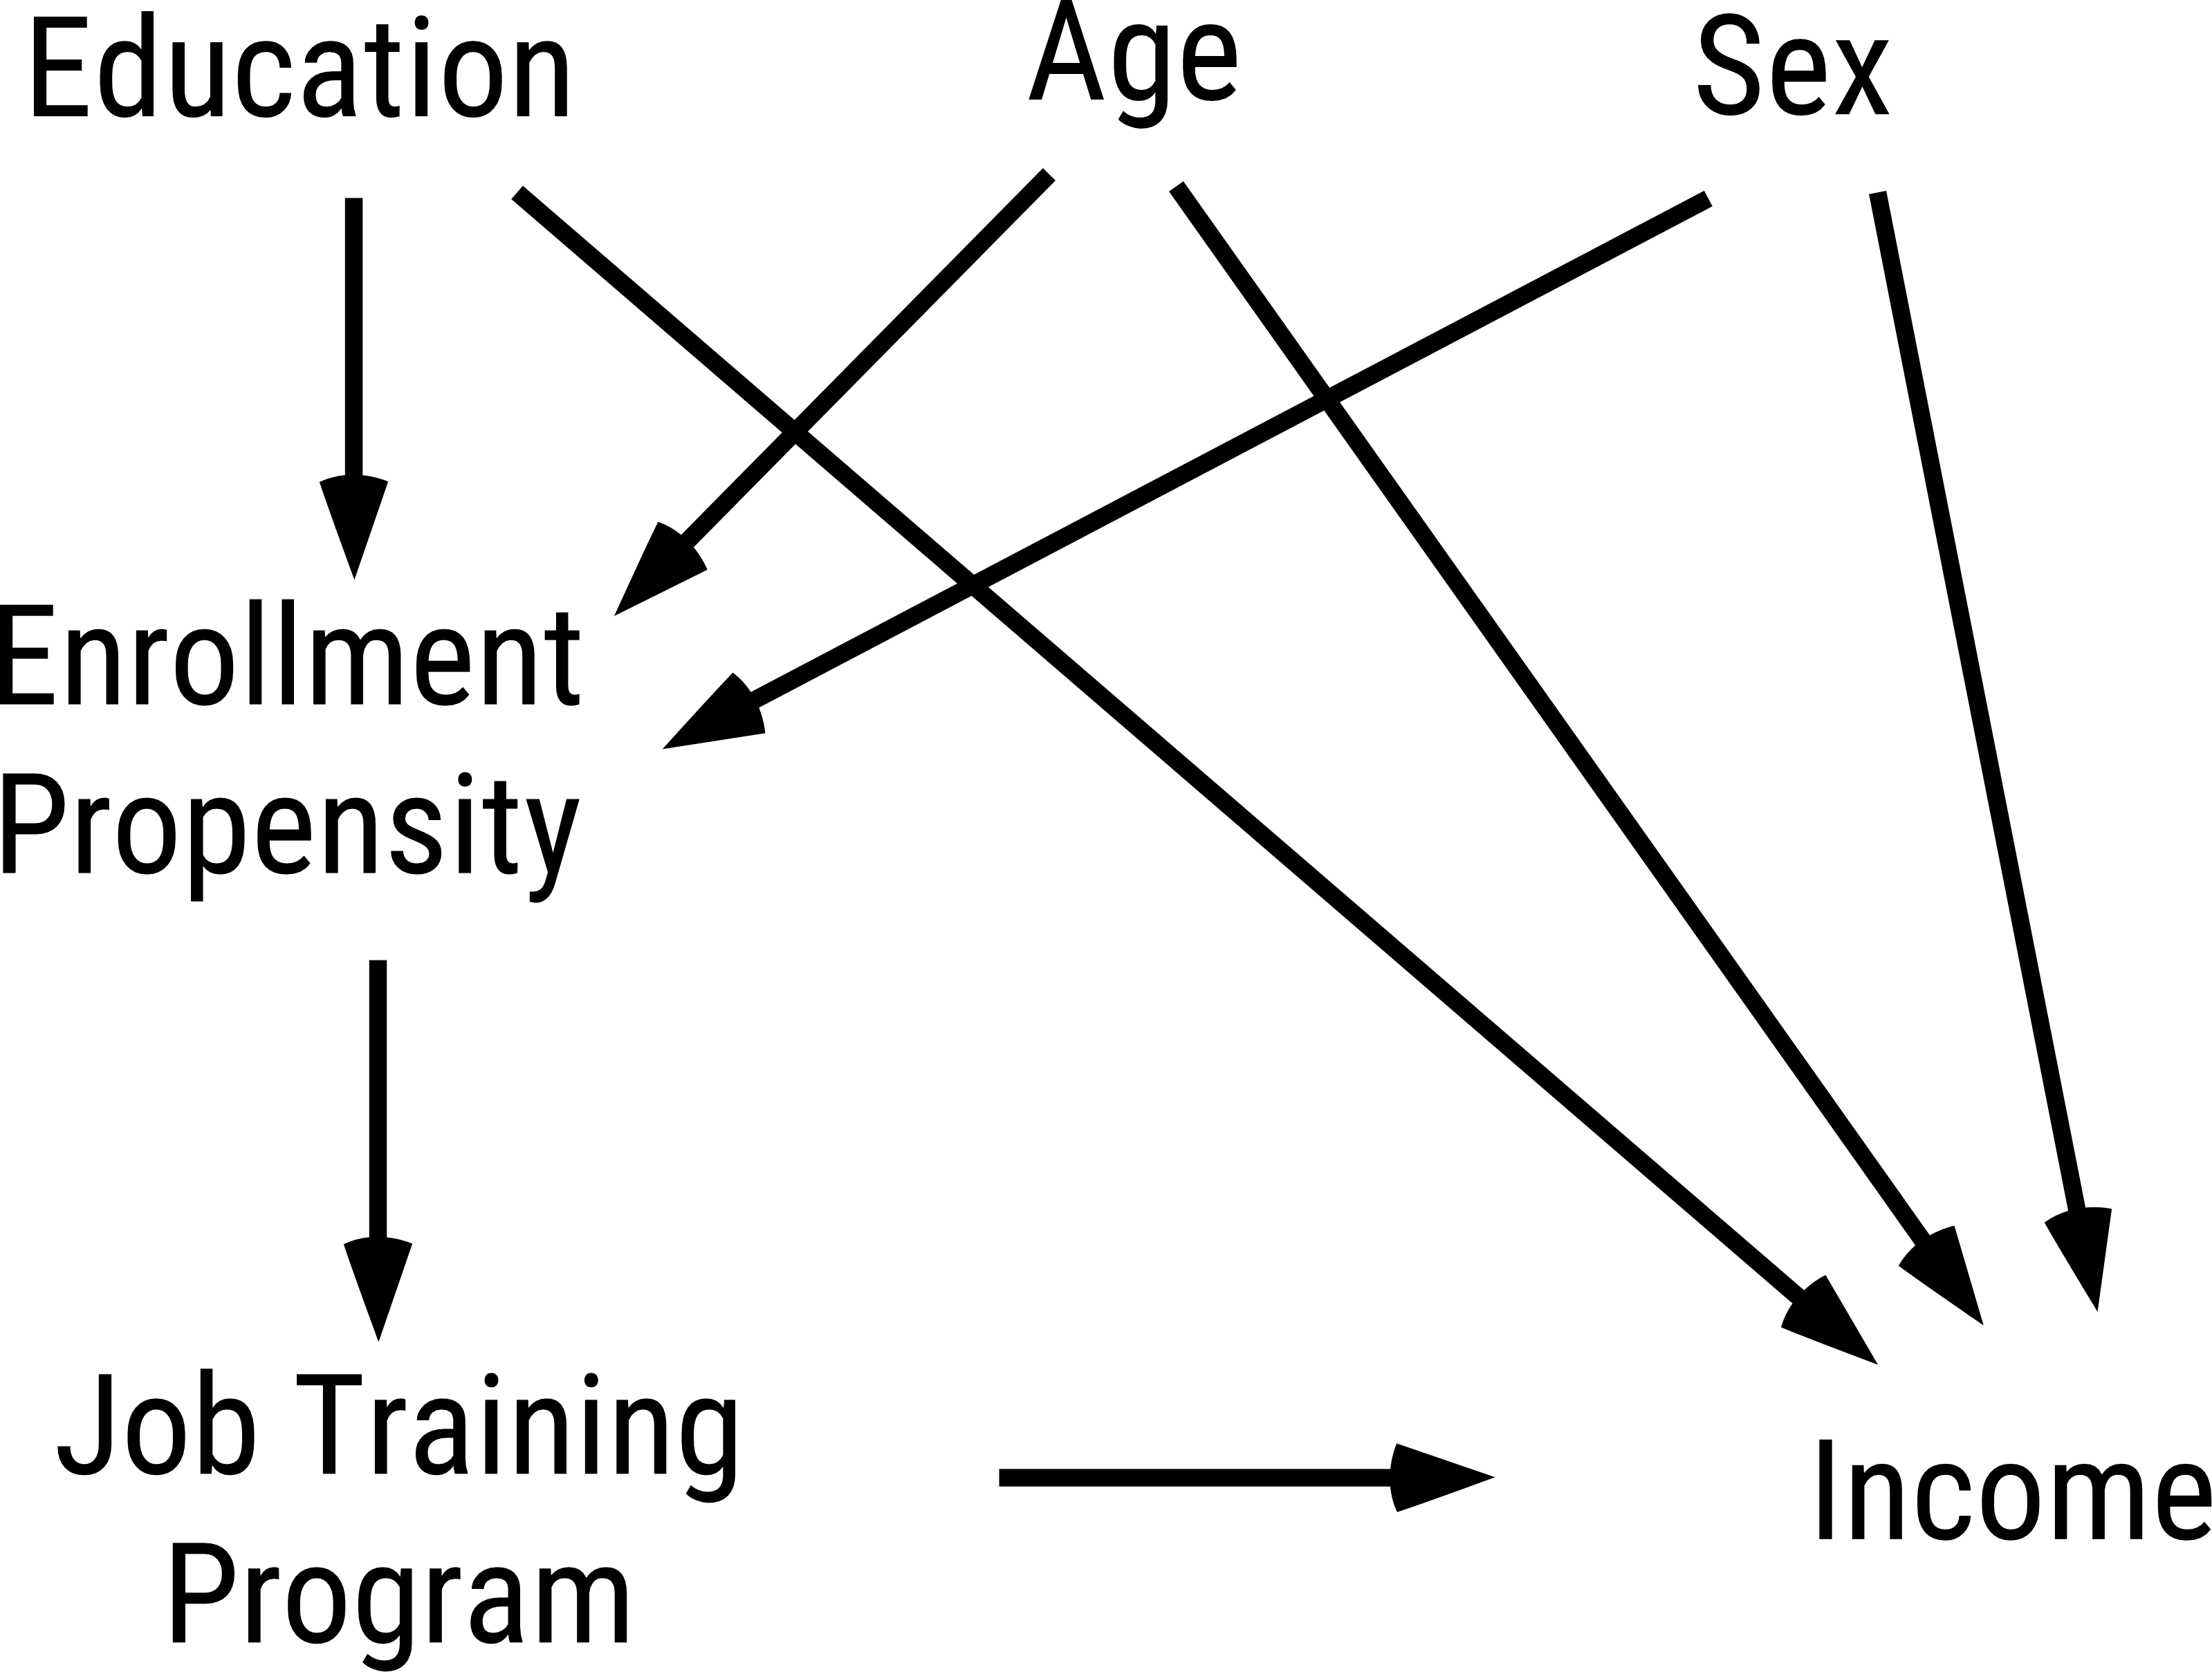
\includegraphics[width=0.5\linewidth]{pictures/dag_matching.png}
			 \caption*{\footnotesize \textit{Notes}: The representation of the directed acyclic graph for propensity score matching comes from \cite{huntington-klein_effect_2021}.}
		\end{figure} 
                
        \paragraph{Case-study and simulation procedure.} We illustrate this issue by simulating a labor training program where the treatment is not randomly allocated \citep{dehejia_causal_1999}. As shown in the directed acylic graph in \Cref{dag_matching}, individuals self-select into the training program and may therefore have different characteristics from individuals who do not choose to enroll. We simulate this type of studies by taking a short-cut. Many simulations found in the applied statistics literature test the performance on matching algorithms by first simulating covariates and then simulating the true but unknown probability of units to be treated. Our goal here is different as we do not want to test the performance of various matching algorithms but rather illustrate how a lack of common overlap in propensity scores can result in a loss of statistical power. We therefore first assign a fraction of individual to the treatment and then simulate the true propensity score variable for treated and control units. For treated units, we draw the propensity scores from a normal distribution $N(\mu_T,\sigma_T)$ and for control units, from $N(\mu_C, \sigma_C)$. Once the true propensity scores are created, we define the potential outcomes of each individual. Here, potential outcomes represent the monthly income (in euros) of the individuals if they undertake the training program or not. The potential outcome of each individual $i$ without treatment adoption, $Y_{i}(0)$, is simulated using the following equation: $Y_i(0)=\text{Wage}\times\text{PS}_i+N(\mu_{\text{N}},\sigma_{\text{N}})$. Wage is the baseline wage, PS$_{i}$ the propensity score of individual $i$ and some noise is drawn from $N(\mu_{\text{N}},\sigma_{\text{N}})$. This equation makes the potential outcomes Y(0) partly different for treated and control units, creating the required common support issue. We then simulate the potential outcomes Y$_i$(1) by adding a constant treatment effect of the training program. The constant treatment effect assumption is made to simplify the illustration of the issue we are interested in. In our simulations, when we make the propensity score matching more stringent, not all treated units can be matched to similar control units. The causal estimand would no longer be the average treatment on the treated if the causal effect was not constant across units.  
        
        Based on this simulation framework, we generate 1000 datasets for each propensity score matching procedure with caliper values ranging from 0 to 1. Parameters values of the simulation are set to make them realistic and can be found \href{https://vincentbagilet.github.io/causal_inflation/Matching.html}{here}. Once units are matched, we simply regress the observed revenue on the treatment indicator.
        
         \begin{figure}[!h] 
			    \caption{Evolution of Bias with the Caliper in Propensity Score Matching, Conditional on Statistical Significance.}
				\label{graph_matching}
			 \centering
\includegraphics[width=0.9\linewidth]{pictures/main_graph_matching_paper.pdf}
			 \caption*{\footnotesize \textit{Notes}: The blue line indicates the average bias for all estimates, regardless of their statistical significance. The orange line represents the inflation of statistically significant estimates at the 5\% level. The caliper is expressed in standard deviation of the propensity score distribution. Details on the simulation are available at this \href{https://vincentbagilet.github.io/causal_inflation/Matching.html}{link}.}
		\end{figure} 
        
        \paragraph{Results.} Figure \ref{graph_matching} indicates that the average bias of estimates, regardless of their statistical significance, decreases with the value of the caliper as units become more comparable. As the caliper decreases, statistically significant estimates start being more inflated than the entire sample of estimates. For large caliper values, units are not comparable enough and confounding bias the effect. For small caliper values, the sample size becomes too small to be able to precisely estimate the treatment effect and exaggeration arises. It is well-known that matching procedure can result in imprecise estimates since it does not use information on outcomes but rather focuses on reducing bias arising from covariates imbalance \citep{rubin2001using}. Yet, in a context of publication bias favoring statistically significant estimates, it may make the method produce misleading claims on treatment effect sizes. 
        
    % REGRESSION DISCONTINUITY DESIGN
    \subsection{Regression Discontinuity Design}
		
        \paragraph{Intuition for the trade-off.} To identify a causal effect, a regression discontinuity approach relies on the assumption that for values close to the threshold, treatment assignment is quasi-random. Under this assumption, individuals just below and just above the threshold would be comparable in terms of observed and unobserved covariates, and only differ in their treatment status. To avoid confounding, the RDD focuses on observations within a certain bandwidth around the threshold and discards observations further away. The effective sample size where the identification of causal effect of the treatment is the most credible differs from the total sample size. For this method, the confounding / exaggeration trade-off is therefore mediated by the size of the bandwidth.
        
        \begin{figure}[!h] 
				\caption{Directed Acyclic Graph for Regression Discontinuity Design Simulations.}
				\label{graph_rdd}
				\centering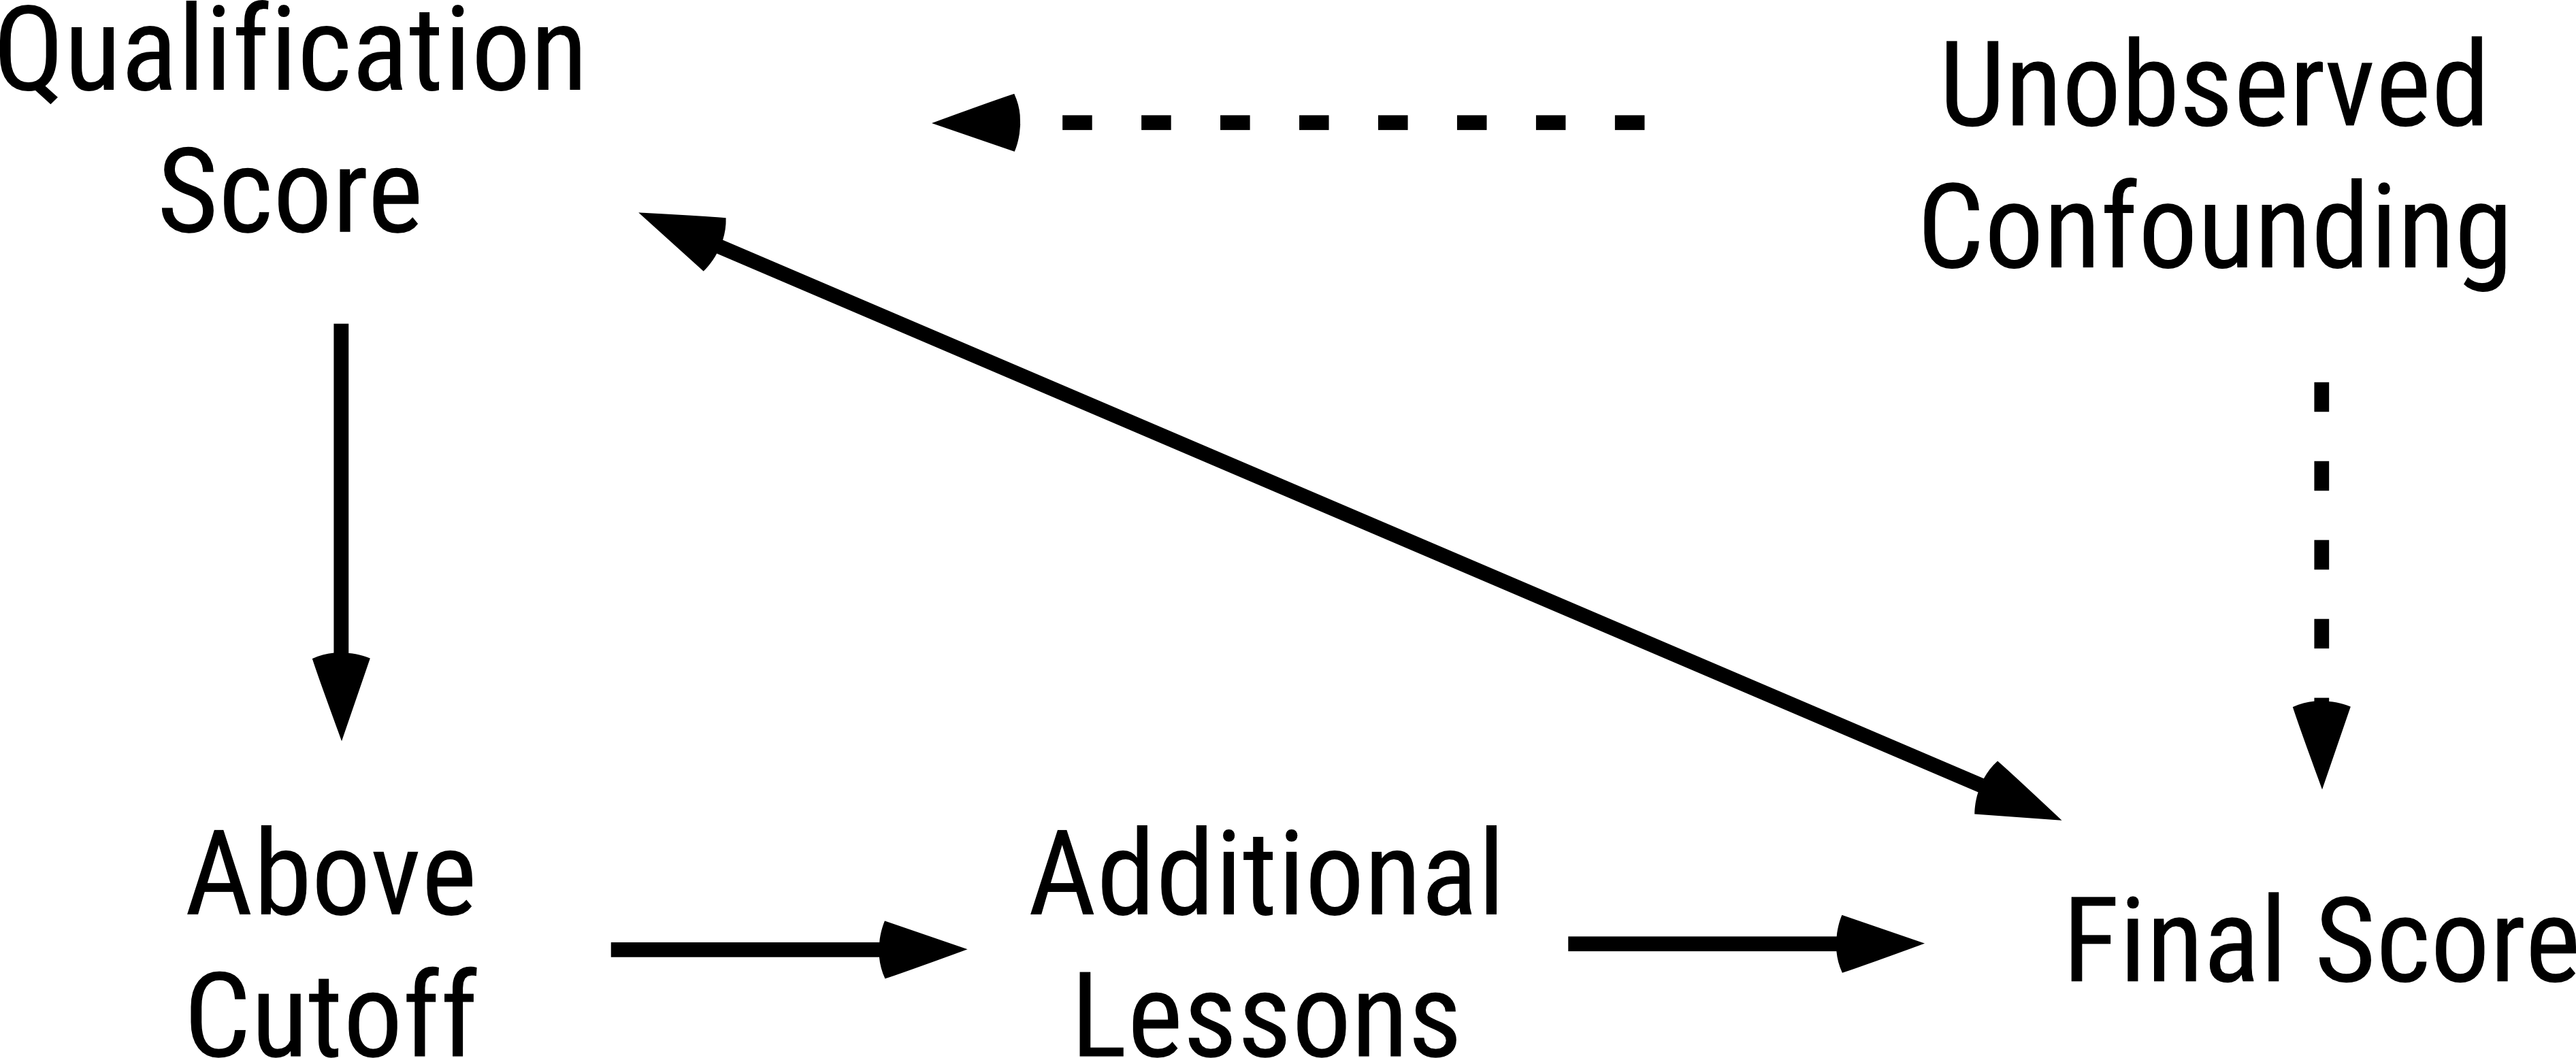
\includegraphics[width=0.7\linewidth]{pictures/dag_rdd.png}
				\caption*{\footnotesize \textit{Notes}: The representation of the directed acyclic graph for the RDD comes from \cite{huntington-klein_effect_2021}.}
		\end{figure} 
        
        \paragraph{Case-study and simulation procedure.} To illustrate this trade-off, we consider a standard application of the sharp RD design in economics of education in which students are offered additional lessons based on the score they obtained on a standardized test \citep{thistlethwaite_regression-discontinuity_1960}. As shown in the directed acyclic graph of \Cref{graph_rdd}, students with initial test scores below a given threshold follow additional lessons while those above do not. Since students far above and far below the threshold may differ along unobserved characteristics such as ability, a RDD estimates the effect of the treatment on final test scores by comparing outcomes of students whose initial test scores are just below and just above this threshold. 
        
        Our simulation framework for RDD is as follows. We assume that if a student $i$ has an initial scores $Qual_{i}$ below a cutoff $C$, she must take additional lessons. The allocation of the treatment $T_i$ is sharp: $T_i = \mathbb{I}[Qual_{i} < C]$. The final scores of students $Final_i$ are correlated with their qualification score $Qual_i$. We further assume that both qualification and final test scores are affected by students' unobserved ability $U_i$ in a non-linear (cubic) way. A large ability has a strong positive impact on test scores. Similarly a particularly low ability strongly impacts test scores negatively. An average ability does not have much impact on test scores. Such a functional form seems realistic. The final test scores $Final_{i}$ are thus defined as follows: $Final_{i} = \alpha^{f} + \beta T_i + \gamma Qual_{i} +  \delta^f f(U_i) + \epsilon_{i}$, where $\alpha^f$ is a constant, $f$ a non linear function and $\epsilon_{i}$ random noise drawn from $\mathcal{N}(0, \sigma_{e})$ noise. The causal parameter of interest is $\beta$. 
        
        To make our simulations realistic, we set the parameters of our simulations based on our reading of \cite{kraft2020interpreting}. They can be found \href{https://vincentbagilet.github.io/causal_inflation/RDD.html}{here}. Given these parameters values, we then generate 1000 datasets with 10,000 observations. For each dataset, we finally estimate the treatment effect by regressing the final score on the treatment status and the qualifying score for different bandwidth sizes. 
        
        \begin{figure}[!h] 
			\begin{center}
				\caption{Evolution of Bias with Bandwidth Size in Regression Discontinuity Design, Conditional on Statistical Significance.}
				\label{graph_rdd}
				
\includegraphics[width=\linewidth]{pictures/main_graph_RDD_paper.pdf}
		        \caption*{\footnotesize \textit{Notes}: The blue line indicates the average bias for all estimates, regardless of their statistical significance. The orange line represents the inflation of statistically significant estimates at the 5\% level. In this simulation, N = 10,000. The bandwidth size is expressed as the proportion of the total number of observations of the entire sample. Details on the simulation are available at this \href{https://vincentbagilet.github.io/causal_inflation/RDD.html}{link}.}			
		        \end{center}
		\end{figure} 
		
		\paragraph{Results.} Figure \ref{graph_rdd} shows that, as the bandwidth around the threshold decreases, the bias of all estimates decreases. This is due to the fact that for large bandwidths, omitted variable arises, while for small bandwidths, treated and control units are very similar in terms of observed and unobserved covariates. However, we observe a U-shape relationship for statistically significant estimates as the bandwidth decreases. For small values of the bandwidth, the statistical power shrinks and statistically significant estimates become inflated. The optimal bandwidth literature describes a similar trade-off but from a different perspective \citep{imbens_optimal_2012}. They consider a bias/precision trade-off while we consider a omitted variable bias / exaggeration bias trade-off due to publication bias favoring statistical significance. 
        
    \subsection{Instrumental Variable Strategy}
    
        \paragraph{Intuition for the trade-off.} Instrumental variable overcomes the issue of unobserved confounding by only considering the exogenous variation in the treatment. When this exogenous fraction of the variation is limited, the instrument can still successfully eliminate confounding on average. However, the IV estimator will be imprecise and statistical power low. In the case of the IV, the confounding / exaggeration trade-off is therefore mediated by the strength of the instrument considered. The weaker the instrument, the more inflated statistically significant estimates will be.
        
        \begin{figure}[!h] 
				\caption{Directed Acyclic Graph for Instrument Variable Simulations.}
				\label{graph_iv}
				\centering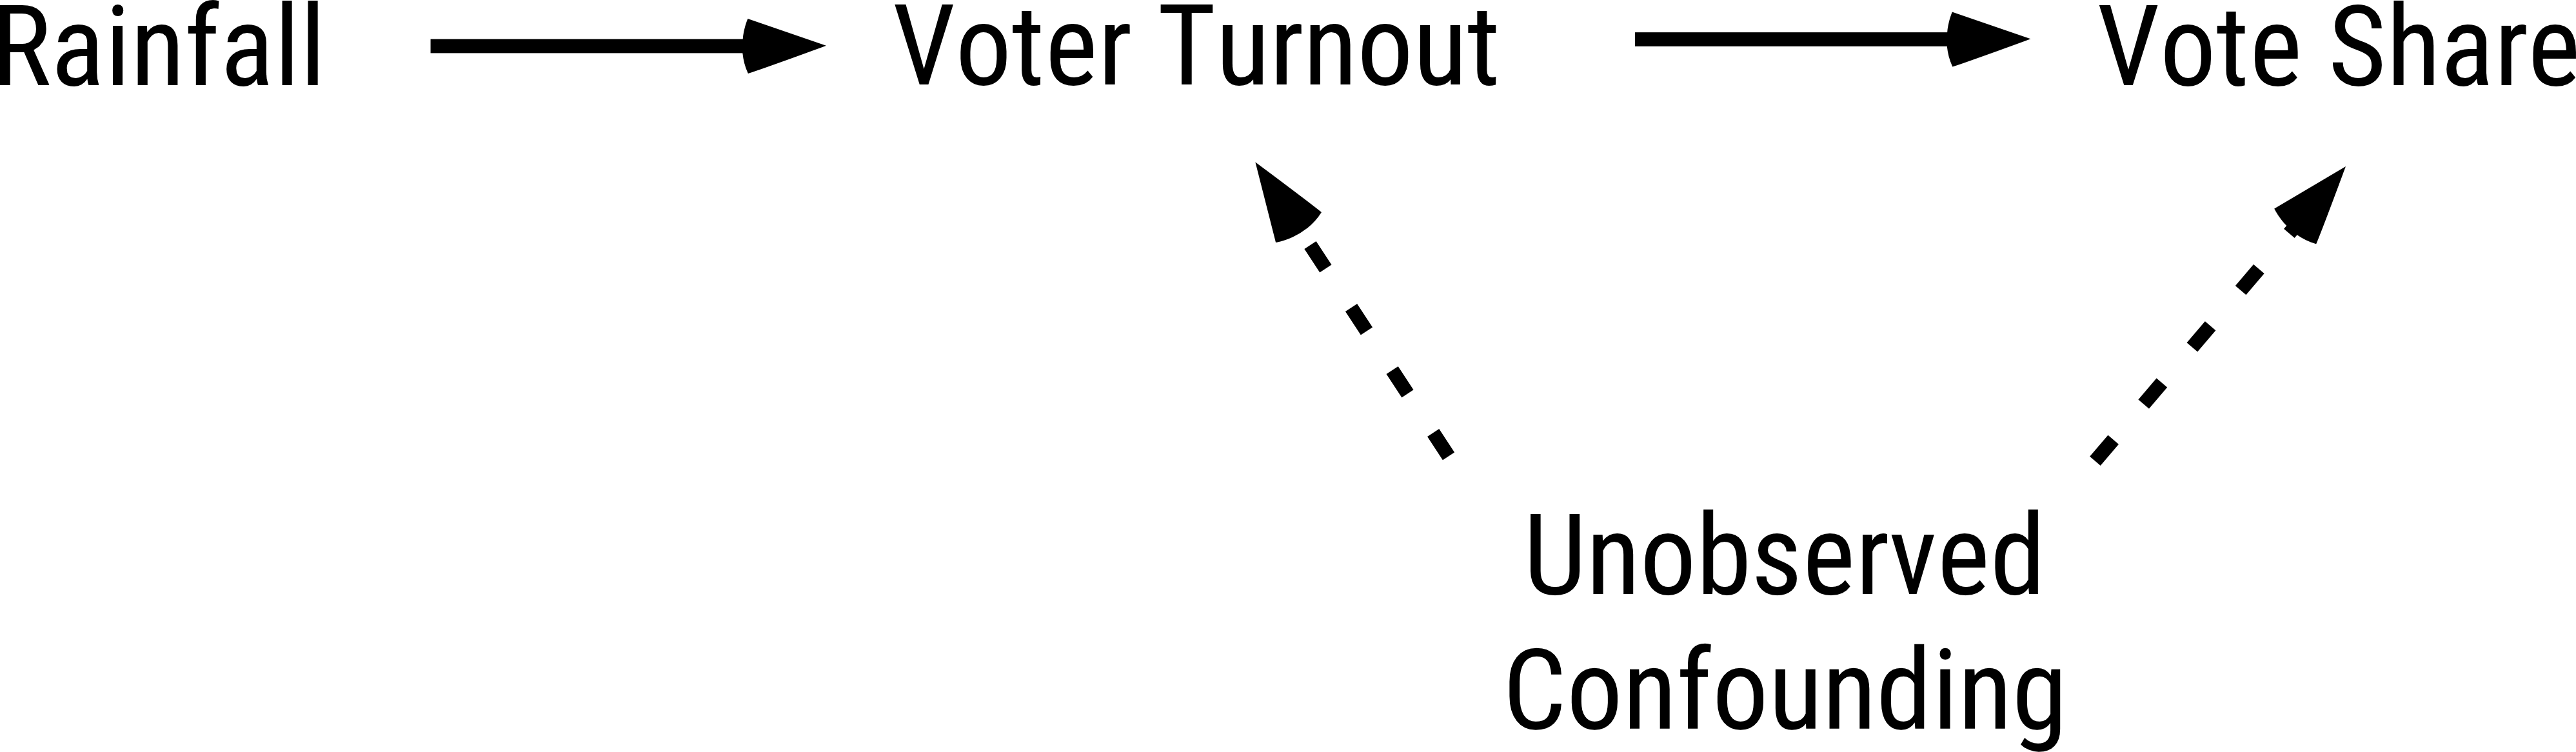
\includegraphics[width=0.8\linewidth]{pictures/dag_iv.png}
		\end{figure} 
        
        
        \paragraph{Case-study and simulation procedure.} To illustrate this trade-off, we take as an example the studies estimating the impact of voter turnout on election results \citep{gomez2007republicans, fujiwara2016habit, cooperman2017randomization}. As shown in \cref{graph_iv}, to avoid the threat of confounding, researchers have taken advantage of exogenous factors that affect voter turnout such as rainfall. In our simulations, we assume that the vote share of a party in location $i$, $Share_i$, can defined such that: $Share_{i} = \alpha + \beta Turnout_{i} + \delta u_{i} + e^{(S)}_{i}$, where $\alpha$ is a constant, $u$ represents an unobserved variable and $e^{(S)} \sim \mathcal{N}(0, \sigma_{e_S})$ noise. The causal parameter of interest is $\beta$. Turnout observations $Turnout_{i}$ are given by the following model: $Turnout_{i} = \gamma + \lambda Rain_{i} + \eta u_{i} + e^{(T)}_{i}$, where $Rain_{i}$ is either a continuous variable (amount of rain in location $i$ on the day of the election) or a dummy variable (whether it rained or not) and $e^{(T)}$ is random noise drawn form $\mathcal{N}(0, \sigma_{e_T})$. We refer to $\lambda$ as the strength of the instrumental variable. 
        
        We discuss in great details how we choose realistic parameters for these two models \href{https://vincentbagilet.github.io/causal_inflation/IV.html}{here}. For each value of the IV strength considered, we create 1000 datasets. We run both a naive ordinary least squares model and a two-stage least squares model to estimate the impact of voter turnout on the vote share of a party.

        \begin{figure}[!h] 
			\begin{center}
				\caption{Evolution of Bias for Statistically Significant Estimates Against Intensity of the Instrument in Instrumental Variable Design.}
				\label{graph_IV}
				
\includegraphics[width=0.9\linewidth]{pictures/main_graph_IV_paper.pdf}
                \caption*{\footnotesize \textit{Notes}: The blue line indicates the average bias for statistically significant IV estimates at the 5\%. The orange line represents the bias of statistically significant OLS estimates at the 5\% level. The strength of the instrumental variable is expressed as the value of the linear parameter linking rainfall to turnout. In this simulation, N = 10,000. Details on the simulation are available at this \href{https://vincentbagilet.github.io/causal_inflation/IV.html}{link}.}
                \end{center}
		\end{figure} 
		
		\paragraph{Results.} Figure \ref{graph_IV} displays, for different IV strengths, the average of statistically significant estimates scaled by the true effect size for both the IV and the naive regression model. When the instrument is strong, the IV will recover the true effect, contrarily to the the naive regression model. Yet, when the IV strength decreases, the exaggeration of statistical significant estimates skyrockets. Even if the intensity of the omitted variable bias is large, for limited IV strengths, the exaggeration ratio can become larger than the omitted variable bias. When the only available instrument is weak, using the naive regression model would, on average, produce statistically significant estimates that are closer to the true effect size than the IV. Of interest for applied research, a large $F$-statistic does not necessarily attenuate this problem. For the parameter values considered here, this phenomenon arises even in cases for which the $F$-statistic is substantially larger than the usually recommended threshold of 10, as illustrated in our \href{https://vincentbagilet.github.io/causal_inflation/IV.html#f-statistic-analysis}{supplementary materials}. 
		
		
	\subsection{Difference-in-Differences Event Study Design}\label{sim_DID}
    
        \paragraph{Intuition for the trade-off.} To avoid confounding, DID event studies take advantage of situations for which we can adjust how the outcome evolved before and after an intervention in a treated group by using the same comparison for an untreated group. The credibility of the method rests on the assumption that the outcomes of the two groups should have evolved similarly had the intervention not occurred. In some cases,  while the number of observations may be large, the proportion of units affected by the intervention might be limited. As a consequence, the number of treated observations is small and the variation available to identify the treatment is limited. In studies using discrete exogenous shocks, a confounding / exaggeration trade-off is thus mediated by the number of observations treated. It does not only concern DID event studies but is particularly salient in this case. 
        
        \begin{figure}[!h] 
				\caption{Directed Acyclic Graph for Difference in Differences Simulations.}
				\label{graph_rdd}
				\centering\includegraphics[width=0.6\linewidth]{pictures/dag_DID.png}
				\caption*{\footnotesize \textit{Notes}: The representation of the directed acyclic graph for the RDD comes from \cite{huntington-klein_effect_2021}.}
		\end{figure} 
        
        \paragraph{Case-study and simulation procedure.} To illustrate this trade-off, we simulate a study on the impact of air pollution reduction on newborn weight of babies. To avoid confounding, one can exploit exogenous shocks to air pollution such as plant closures, creation of a low emission zone or of an urban toll. We simulate our analysis at the zip code and monthly levels and focus on the example of toxic plant closures \citep{currie2015environmental}. We consider that the average birth weight in zip code $z$ at time period $t$, $bw_{zt}$, depends on a zip code fixed effect $\zeta_z$, a time fixed effect $\tau_t$, and the treatment status $T_{z,t}$, which is equal to one if a plant closed in this period and 0 otherwise. The average birth weights $bw_{zt}$ is defined as follows: $bw_{z,t} = \alpha + \beta T_{z, t} + \zeta_z + \tau_t + \epsilon_{z,t}$. To simplify further the simulations, we assume that the treatment allocation is not staggered and its effect is constant in time and homogeneous across zip codes. We vary in the simulations the proportion of zip codes affected by toxic plant closings.

       The parameters values of our simulations are inspired by \citep{currie2015environmental} and can be found \href{https://vincentbagilet.github.io/causal_inflation/DID.html}{here}. For a fixed sample size of 120,000 observations, we generate 1000 datasets for an increasing number of treated observations and run our two-way fixed effects model.
        
        \begin{figure}[!h] 
			\begin{center}
				\caption{Evolution of Bias for Statistically Significant Estimates against the Number of Treated Observations in Difference-in-Differences Event Study Design.}
				\label{graph_DID}
				
\includegraphics[width=0.9\linewidth]{pictures/main_graph_DID_paper.pdf}
                \caption*{\footnotesize \textit{Notes}: The blue line indicates the average bias for statistically significant estimates at the 5\%. In this simulation, N = 120,000. Details on the simulation are available at this \href{https://vincentbagilet.github.io/causal_inflation/DID.html}{link}.}
			\end{center}
		\end{figure} 
		
		\paragraph{Results.} Even though the actual sample size is extremely large in our example, if the number of treated observations is small, the exaggeration can be important, as shown in \Cref{graph_DID}. A very large number of observations does not necessarily prevent the exaggeration issue to arise. The intuition behind this result can be compared to the case of a complete randomized controlled trial where, for fixed sample size, the statistical power is maximized when units are equally allocated to treatment and control groups.
		
%-----------------------------------------------------------------------------

% PRACTICAL RECOMMENDATIONS

%-----------------------------------------------------------------------------

\section{Practical Recommendations} \label{discussion}

% HOOK OF THE SECTION
    Once we realize that causal methods can produce inflated estimates when the study is under-powered, how can we address this problem? Even though it does not produce uninflated estimates, reporting power calculations enables to evaluate the risk of exaggeration for a study. In this section, we present a workflow to evaluate and report the power of a study before and after its implementation. We then discuss how changing our attitude towards statistical significance and replicating studies can help limit this issue.

% SOLUTIONS BEFORE WE FULLY ANALYZE THE DATA
\subsection{Before Analyzing the Data}

    In randomized controlled trials, presenting statistical power calculations before running the experiment is not only an established practice but also a requirement  \citep{duflo_using_2007, mcconnell_going_2015, athey_econometrics_2016}. Power is however rarely reported in observational studies, despite the availability of specific power formulas for some causal inference methods \citep{freeman_power_2013, cattaneo_power_2019}. Two main reasons could explain this limited reporting of power calculations. First, we do not directly control the data collection process in our research projects. Second, we may fear that available power formulas are not flexible enough to capture the complexity of their design. On top of these reasons, there is a lack of guidance on how to design well-powered observational studies. In causal inference textbooks, very few pages are devoted to the topic \citep{angrist_mostly_2009, angrist_mastering_2014, imbens_causal_2015, cunningham_causal_2021}. To the best of our knowledge, only two textbooks discuss the matter in depth \citep{shadish_experimental_2002, huntington-klein_effect_2021}.
    
    
    Simulating the design of an observational study is a solution to overcome these limits \citep{hill_bayesian_2011, gelman_regression_2020, black_simulated_2021}. Similarly to what we did in the previous section, the goal of this approach is to simulate the data generating process of the study from scratch. It requires thinking about the distribution of the variables and their relationships. External information found in previous studies can help guide the simulation process to make it more realistic. If the relationships among covariates are too complex to emulate, a second approach starts from an existing dataset to which a simulated treatment and potential outcomes are added\footnote{In the future version of the paper, we will explain how we can easily simulate from scratch the study by \cite{card_using_1993}. For now, examples of simple simulations are available on our \href{https://vincentbagilet.github.io/causal_inflation/}{companion website}.}.

    When simulations indicate that statistical power is low, additional data could be collected or the statistical model could be expanded to increase precision. In any case, it should not stop from carrying out a research project. Simulation results rest on the way the data generation process was modeled and it can be difficult to gauge the amount of noise present in data before actually analyzing them. The two actual benefits of a prospective simulation procedure are to think about factors that affect power and not to be mislead by statistically significant estimates if power is low. 

% SOLUTIONS AFTER ANALYZING THE DATA
\subsection{Once the Main Analysis is Completed}

    Once we have obtained a statistically significant estimate for the treatment of interest, we still need to think about the statistical power of the study to check whether the magnitude of our estimate is trustworthy. A \textit{retrospective} power analysis helps evaluate whether the design of the study would  produce uninflated statistically significant estimates if the true effect was smaller than the observed estimate \citep{gelman_beyond_2014, ioannidis_power_2017, stommes_reliability_2021}.
    
    We illustrate how a retrospective analysis works by taking the example of \cite{card_using_1993} on the relationship between human capital and income. He finds that an additional year of education, instrumented by the distance of growing near a four-year college, causes a 13.2\% average increase in wage. The associated standard error is 5.5\%. As noted by the author himself, the estimate is very imprecise: if the true causal effect was slightly smaller than the observed estimate, the study would very likely be under-powered. For instance, imagine that prior evidence suggests that the true effect could be to closer a 10\% increase in wage. Computing the statistical power of the study only requires to draw many estimates from a normal distribution centered around the hypothesized true effect of 10\% and with a standard deviation equal to the 5.5\% standard error obtained in \cite{card_using_1993}. Concretely, one proceeds as if they were able to replicate the study many times under the assumption that the true effect is different from the observed estimate. The proportion of sampled estimates that are statistically significant at the 5\% level, 44\% in this case, is the statistical power. The inflation of significant estimates is then computed as the average ratio of the values of statistically significant estimates over the assumed true effect size: these estimates would be 1.5 times too large on average. 
    
    For a retrospective power analysis to be useful, it is therefore necessary to make informed guesses about the range of plausible effect sizes. Such guesses can be based on results from meta-analyses or previous studies with a convincing design (e.g., a large randomized controlled trial). When such information is not available, power calculations can be run for a range of smaller but credible effect sizes\footnote{We are currently working on the adoption of two existing approaches that could help address the potential inflation of statistically significant estimates. 
    In a series of articles, \cite{zwet_proposal_2021, zwet_significance_2021} and \cite{zwet_statistical_2021} present a Bayesian procedure to shrink statistically significant estimates based on a corpus of estimates from prior studies.
    The second approach consists in carrying out quantitative bias analyses to evaluate whether the threat of unobserved confounding requires a restrictive causal approach. \cite{rosenbaum_observational_2002}, \cite{oster_unobservable_2019} and \cite{cinelli_making_2020} have developed different methods to run sensitivity analyses. They could be paired with power calculations to better evaluate the hidden bias / power trade-off of competing research designs. For instance, if a sensitivity analysis reveals that a simple selection on observables strategy is very robust to omitted variable bias, one may avoid using an IV model since it has a higher chance to produce inflated estimates.}.
    
    Results from power and exaggeration calculations would not only be highly informative but could also be reported very concisely in the robustness section of articles. \texttt{R} and \texttt{Stata} packages have been developed \citep{timm_retrodesign_2019, linden_retrodesign_2019} to easily implement retrospective power analyses. 

% GENERAL RECOMMENDATIONS
\subsection{Attitude Towards Statistical Significance and Replication}

    General changes in scientific practices could also limit the inflation of statistically significant estimates in under-powered studies. As shown in our simulations, if estimates were not filtered by their statistical significance, even under-powered studies would on average recover the true effect. The publication bias arising from dichotomizing evidence according to $p$-values has long been criticized in many disciplines but has seen a revival with the recent replication crises in psychology, medicine and social sciences. Many researchers advocate abandoning statistical significance as a measure of a study's quality \citep{mcshane_abandon_2019}. This would essentially eliminate the trade-off described in this paper.

    To be effective, this change in attitude towards statistical significance should be paired with an effort to replicate studies \citep{christensen_transparency_2018}. Replications, even of low powered studies, would eventually enable to build the distribution of the causal estimand of interest. Meta-analyzes would then reduce the uncertainty around the true value of the causal estimand by pooling estimates \citep{hernan_causal_2021}. 

    Finally, the inflation of statistically significant estimates can be limited by considering confidence intervals as compatibility intervals \citep{shadish_experimental_2002, amrhein_inferential_2019, romer_praise_2020}. The width of these intervals gives a range of effect sizes compatible with the data. Confidence intervals will be wide in under-powered studies signaling that point estimates should not be taken at face value, even if statistically significant.

%-----------------------------------------------------------------------------

% CONCLUSION

%-----------------------------------------------------------------------------

\section{Conclusion} \label{conclusion}

    Causal identification strategies have undoubtedly participated in making empirical analyses more credible \citep{angrist_credibility_2010}. To avoid confounding, they only exploit the exogenous part of treatment variation. In this paper, we argue that the same aspect that makes causal identification strategies credible can create another type of bias. Not only the lack of precision makes it more difficult to precisely get a sense of the magnitude of the actual effect but it also increases the probability of published estimates to be inflated. The confounding / exaggeration trade-off we highlight in this paper manifests itself along different dimensions for each identification strategy. A systematic reporting of statistical power calculations in observational studies could help gauge the risk of falling into this low power trap. 

%-----------------------------------------------------------------------------

% BIBLIOGRAPHY

%-----------------------------------------------------------------------------

\setlength\bibsep{0pt}
\bibliographystyle{c}
\bibliography{causal_inflation.bib}

\end{document}
